\setchapterpreamble[u]{\margintoc}
\chapter{Optimization of indoor LiDAR scans}
\labch{lidar_optimization}
\label{sec:lidar_optimization}

\section*{About this chapter}

This chapter presents a synthetic GPU-based LiDAR scanner. It is parameterized to emulate a large number of sensor models, ranging from airborne to terrestrial scanning. The approach is massively parallelized in the GPU to solve millions of collisions with a reduced response time, even simulating multiple returns for forestry environments. This work is mainly intended for the rapid generation of datasets consisting of hundreds of millions of points for Deep Learning. The conducted tests show that the proposed approach outperforms a sequential approach, and its capabilities on the generation of large datasets were shown to improve previous work. 

\begin{marginfigure}[3cm]
    \centering
    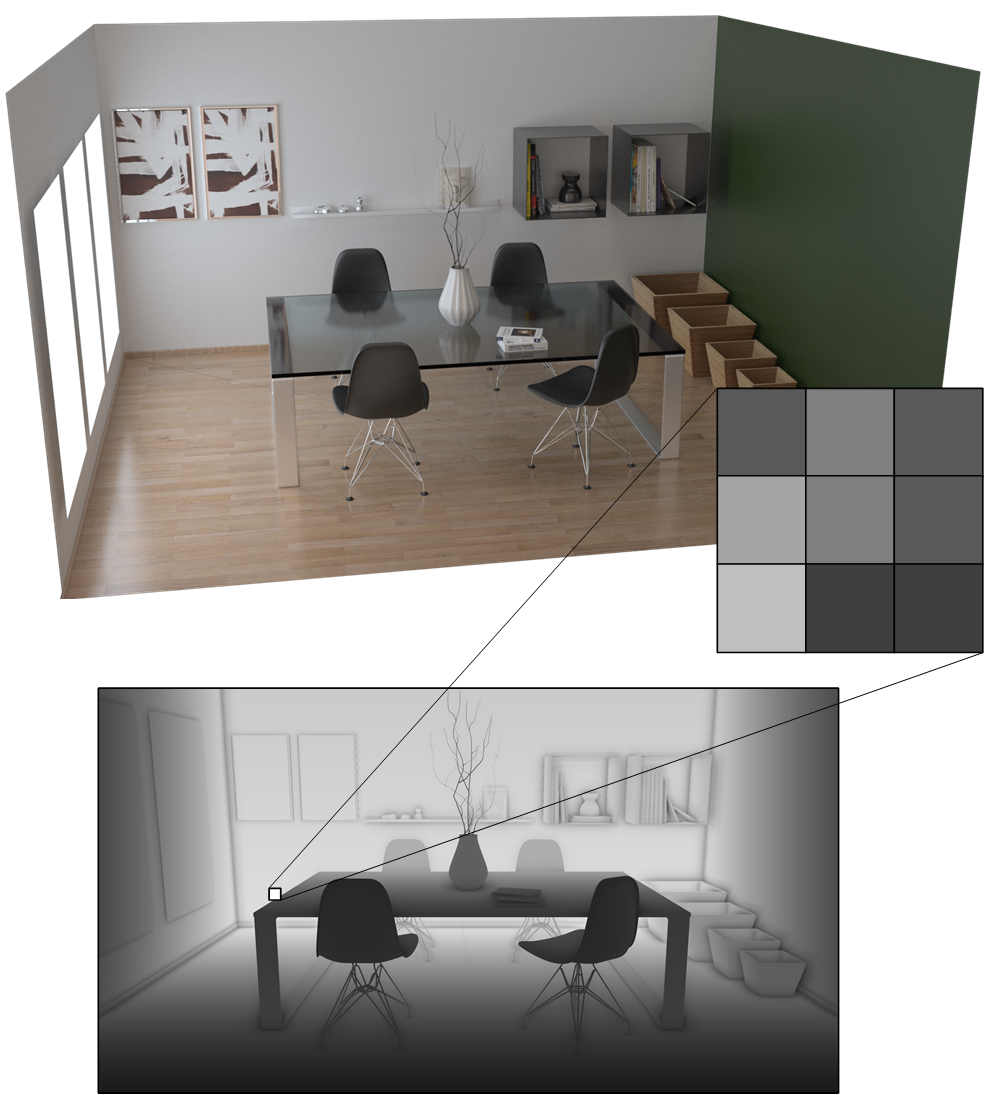
\includegraphics[width=\linewidth]{figs/lidar_simulation/depth_buffer.png}
	\caption{Depth buffer of a 3D scene, as proposed in previous LiDAR simulations. }
	\label{fig:depth_buffer_lidar}
\end{marginfigure}
Another key factor is the use of procedural 3D environments; scenes modelled by professionals can be utilized for generating a few datasets from several viewpoints, whereas those governed by generation rules lead to constructing large datasets from different environments. Besides TLS, which is by far the most studied kind of LiDAR sensor, this chapter is also intended for describing how to simulate aerial surveys considering both sensor errors and surface properties. In comparison with previous work, collisions are solved using state-of-the-art ray-tracing data structures, instead of solving it through a \textit{z}-buffer of limited resolution (Figure \ref{fig:depth_buffer_lidar}). Consequently, this piece of software is able to construct high-quality point clouds with low latency. Nevertheless, working in the image space is sometimes required; for instance, Deep Learning models are easier to operate in images than over 3D point clouds without losing precision on them (e.g., by voxelizing).

In comparison with previous work, the main contributions of this chapter are the generation of large labelled LiDAR datasets using procedural scenarios as input. These are obtained in a reduced response time, following a physically-based interaction, while a sequential approach requires several minutes, even hours, for solving complete scans of a whole target area. The complete procedure is depicted in Figure \ref{fig:lidar_overview}. 

\section{On the optimization of TLS scans}

